\documentclass{article}

\usepackage{amsmath}
\usepackage{amssymb}
\usepackage{graphicx}
\usepackage{float}
\usepackage{epstopdf}
\usepackage{hyperref}
\hypersetup {
	urlcolor=blue
}
\graphicspath{./}

\title{Categorizing Commodities by Price Reconstruction}
\author{Bennet Montgomery 20074049}
\date{2019-03-12}

\begin{document}
	\maketitle
	
	\section*{Abstract}
	This experiment was conducted in order to determine the categorization of two sets of commodity prices using PCA. A PCA was conducted on two datasets $z1$ and $z2$ provided by the professor. The error of reconstructing these two datasets was compared to determine which one was a set of food based commodities and which one was a set of basic material commodities. Ultimately, $z1$ was determined to be the dataset most likely to be composed of basic material commodities and $z2$ was determined to be the dataset most likely to be composed of food based commodities. 
	\section*{Introduction}
	This experiment was conducted to determine if two sets of commodity pricing data could be grouped into a set of food based commodities and basic material commodities with no information other than the commodity prices over a period of time and PCA based data reconstruction. In general, commodities are often grouped into classes such as food based, raw material, or fuel. In this case, we were specifally concerned with food based and basic material commodities. One of the cheapest basic material commodities is wood pulp, which is valued at 0.88 USD/kg; on the other hand palladium, one of the most expensive basic material commodities, is valued at more than 48000 USD/kg.$^{[1, \hphantom{a} 2]}$ Comparing this to food based commodities where one of the cheapest commodities, rice, is 0.41 USD/kg and one of the most expensive commodities, arabica coffee, is 213.85 USD/kg, we see much less price range in food based than basic material commodities.$^{[3, \hphantom{a} 4]}$ We can use this difference in magnitude of variation to determine which of the $z1$ and $z2$ datasets was food based commodities and which was basic material commodities. If one of the datasets is for food based and the other is for basic material commodities, the errors of reconstruction using PCA should be observably more erratic in one of the datasets than the other as basic material commodities have a very high magnitude of price range making reconstruction off of a mean price difficult. The dataset with the more erratic and greater average errors of reconstruction is the dataset of basic material commodities.
	
	\section*{Methods}
	The number of principal components used to reconstruct values of each dataset was derived through the SVD of the input datasets using $pcaprelim$ and applying the formula for $\rho$ to the resulting matrix $\Sigma$, $\rho = \frac{t_k}{t_n}$ where $t_k$ is the sum of the first $k$ singular values of $\Sigma$ and $t_n$ is the sum of all singular values of $\Sigma$. The value of $k$ for which approximation coverage was closest to 50\% but not above 60\% was then used in approximation with $pcaapprox$. The root mean standard error of reconstruction was then calculated for both datasets, and the dataset with the more erratic RMSE values was designated as the set of basic material commodities.
	
	\section*{Results}
	The first ten singular values of $\Sigma$ calculated for dataset z1 were:
	\begin{table}[ht]
		\centering
		\begin{tabular}{ c | c }
			\hline
			\hline	
			k value & $\sigma _k$ \\
			\hline
			1 & 480.1588 \\
			2 & 365.3733 \\
			3 & 345.1872 \\
			4 & 244.1168 \\
			5 & 217.3503 \\
			6 & 164.3624 \\
			7 & 158.8629 \\
			8 & 122.6255 \\
			9 & 111.8564 \\
			10 & 105.5666 \\
			\hline
		\end{tabular}
	\end{table}
	\\The first ten singular values of $\Sigma$ calculated for dataset z2 were:
	\begin{table}[ht]
		\centering
		\begin{tabular}{ c | c }
			\hline
			\hline	
			k value & $\sigma _k$ \\
			\hline
			1 & 620.8051 \\
			2 & 365.4937 \\
			3 & 306.6411 \\
			4 & 175.5838 \\
			5 & 158.8907 \\
			6 & 143.9413 \\
			7 & 109.3216 \\
			8 & 103.9568 \\
			9 & 94.4101 \\
			10 & 70.8589 \\
			\hline
		\end{tabular}
	\end{table}
	\\The optimal value of $k$ to use for approximation for was found to be at $k = 4$ for $z1$ with an approximation coverage percentage of 52.79\% and $k = 3$ for $z2$ with an approximation coverage percentage of 53.56\% (Figure 1).
	\begin{figure}[H]
    	\centering
    	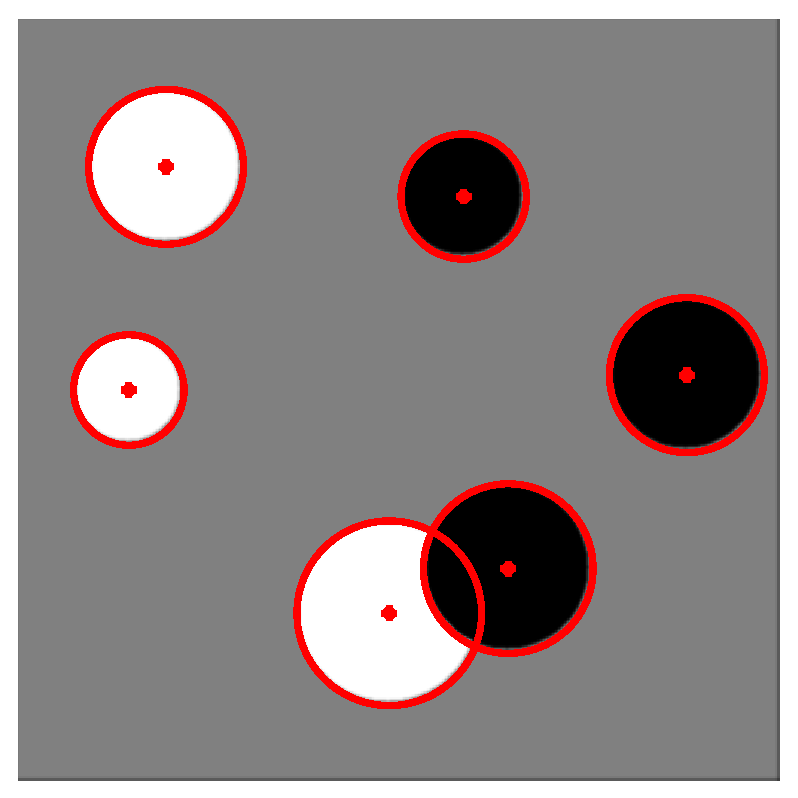
\includegraphics{figure1}
    	\caption{Approximation coverage percentage trend over $k$ values. The optimal $k$ values for $z1$ and $z2$ were found to be 4 and 3 with approximation coverages of 52.79\% and 53.56\% respectively.}
	\end{figure}
	Calculation of the RMSE of reconstruction yielded a much more variable reconstruction error and higher average error of approximation when approximating $z1$ than when approximating $z2$. The difference between the highest and lowest errors of reconstruction for $z1$ was 10.83, the difference between the highest and lowest errors of reconstruction for $z2$ was 6.6. The average reconstruction error of $z1$ was 9.1424, the average reconstruction error for $z2$ was 8.1753 (Figure 2).
	\begin{figure}[H]
		\centering
		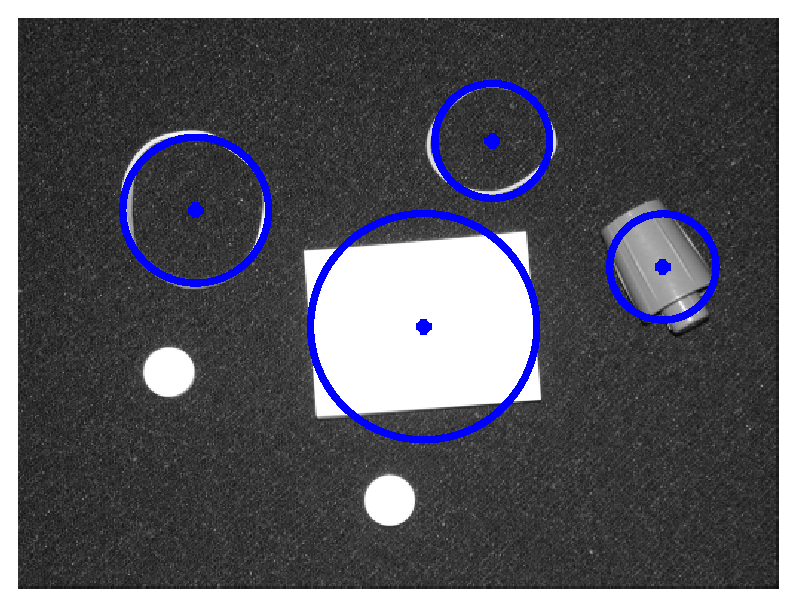
\includegraphics{figure2}
		\caption{Note the high variability in error of reconstruction for $z1$ compared to $z2$. The difference between the highest error of reconstruction for $z1$ (16.46) and the lowest error of reconstruction for $z1$ (5.635) was 10.83. The difference between the highest error of reconstruction for $z2$ (12.04) and the lowest error of reconstruction for $z2$ (5.44) was 6.60. The average RMSE of reconstruction of $z1$ was 9.1424, the average RMSE of reconstruction for $z2$ was 8.1753.}
	\end{figure}
	\section*{Discussion}
	The dataset $z1$ was the dataset with both the more erratic errors of reconstruction and the dataset with the higher average errors of reconstructon. From this, we can say that $z1$ is the dataset more likely to be composed of basic material commodities. The reason that this method for determining commodity set type is that the algorithm for approximation will have greater trouble approximating basic material commodities because of the relatively large range of prices per mass of basic material commodities compared to food based commodities. Basic material commodities with prices close to the mean price trend will be reconstructed with much less error than commodities with prices either much lower or much higher than the mean price trend. Food commodities on the other hand have a much lower variation in price, and therefore outliers relative to the mean trend are not as hard to approximate as outliers to the mean trend for basic material commodities. 
	\section*{References}
	1. N.a. Wood Pulp Monthly Price - US Dollars Per Metric Ton [Internet]. 2019-01 [cited 2019-03-12]. \url{https://www.indexmundi.com/commodities/?commodity=wood-pulp&months=120}\\\\
	2. N.a. Palladium Futures End of Day Settlement Price [Internet]. 2019-03-12 [cited 2019-03-12]. \url{https://www.indexmundi.com/commodities/?commodity=palladium}\\\\
	3. N.a. Rice Monthly Price - US Dollars Per Metric Ton [Internet]. 2019-01 [cited 2019-03-12]. \url{https://https://www.indexmundi.com/commodities/?commodity=rice}\\\\
	4. N.a. Coffee Futures End of Day Settlement Price [Internet]. 2019-03-12 [cited 2019-03-12]. \url{https://https://www.indexmundi.com/commodities/?commodity=other-mild-arabicas-coffee}\\\\
\end{document}